\chapter{Appendix}\label{sec:appendix}

\section{Experimental setup and tools}
\subsection*{Fitting fluorescence oscillations - oscillating probe under a fixed Gaussian beam}\label{app:pl_osc}
Assume the spatial intensity profile of the focused laser spot is characterized by a fundamental Gaussian distribution:
\begin{equation}
    \centering
    I(x) = I_{max} \exp\left(-\frac{2(x - x_c)^2}{w_0^2}\right),
\end{equation}

where $x_c$ is the spatial center of the laser focus, $w_0$ is the $1/e^2$ beam waist radius. The position of an emitter oscillating harmonically along the $x$-axis is given by:
\begin{equation}
    \centering
    x(t) = x_{eq} + \Delta x \sin(2 \pi f_{tf} t + \beta),
\end{equation}
where $x_{eq}$ is the equilibrium position of the emitter, $\Delta x$ is the physical oscillation amplitude, and $f_{tf}$ the frequency of the tuning fork. Substituting the kinematic equation into the intensity profile yields the time-dependent intensity observed by the emitter:
\begin{equation}
    \centering
    I(t) = I_{max} \exp\left(-\frac{2}{w_0^2}\left(x_{eq} - x_c + \Delta x \sin(2 \pi f_{tf} t + \beta)\right)^2\right)
\end{equation}

The exponent of the derived physical model can be factored to isolate the static offset and the dynamic oscillation:
\begin{equation}
    \centering
    P(t) = -\left( \frac{\sqrt{2}(x_{eq} - x_c)}{w_0} + \frac{\sqrt{2}\Delta x}{w_0} \sin(2 \pi f_{tf} t + \beta) \right)^2
\end{equation}

The fitting function used has the form,
\begin{equation}\label{eq:grad_fit}
    \begin{split}
    y &= C \cdot exp(P) \\
    P(t) &= -(A + B \sin(2 \pi f_{tf} t + \beta))^2
    \end{split}
\end{equation}

Comparing these yields the following equivalences:
\begin{equation}
    \centering
    A = \frac{\sqrt{2}(x_{eq} - x_c)}{w_0}
\end{equation}
\begin{equation}
    \centering
    B = \frac{\sqrt{2}\Delta x}{w_0}
\end{equation}

Rearranging the expression for $B$ allows for the direct calculation of the oscillation amplitude $\Delta x$:
\begin{equation}
    \centering
    \Delta x = \frac{B \cdot w_0}{\sqrt{2}}
\end{equation}
To resolve $\Delta x$ in nanometers, the parameter $w_0$ must be defined. For a diffraction-limited optical system, the beam waist depends fundamentally on the emission wavelength ($\lambda$) and the numerical aperture ($\text{NA}$) of the objective. If the objective lens is fully overfilled (yielding a truncated Gaussian approximating an Airy disk), the $1/e^2$ beam waist can be approximated by:
\begin{equation}
    \centering
    w_0 \approx \frac{0.42 \lambda}{\text{NA}}
\end{equation}

Substituting this approximation into the amplitude equation yields the final formula\cite{zhangGaussianApproximationsFluorescence2007}:
\begin{equation}
    \centering
    \Delta x \approx \frac{0.42 \cdot B \cdot \lambda}{\sqrt{2} \cdot \text{NA}}
\end{equation}


This derivation assumes strictly one-dimensional motion across the center of the beam spot and neglects axial ($z$-axis) variations in the point spread function. Furthermore, the constant $0.42$ is an ideal diffraction-limited approximation. Aberrations, incomplete pupil filling, wrong estimation of NA, beam shaping due to a emitter in a waveguide, etc. will expand $w_0$, meaning the calculated $\Delta x$ using the ideal formula represents a theoretical lower bound for the true physical amplitude.

\subsection*{Trigger level sweep for gradiometry triggering}\label{app:phase_volt}
In this system the $V0$ and $V1$ are set to have a constant difference of \qty{200}{\milli\volt}, such that $V0 = V1 + \qty{200}{\milli\volt}$ (see \cref{fig:gradiometry}). In \cref{fig:phase_volt}, $V0$ is swept and the gradiometry phase collected for a fixed $t_0$. This is similar to a $t_0$ sweep but with limited range and only serves the purpose to ensure that the full measurement is optimized by reducing dead time. Setting the trigger level close to the value that gives maximum phase ensures a small $t_0$ time and therefore an oscillation period is not wasted.
\begin{figure}[h]
    \centering 
    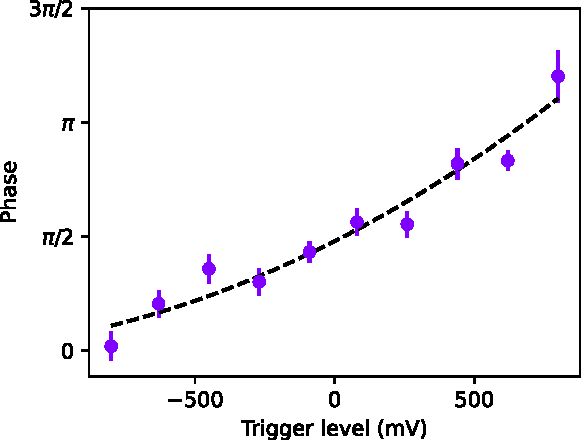
\includegraphics[width=0.95\textwidth]{../figures/phase_volt.pdf}
    \caption[Trigger level sweep for gradiometry]{Trigger level sweep for gradiometry. Triggering by the mechanical oscillation is done with a rearm ($trig0$ or $V0$) and trigger ($trig1$ or $V1$) levels which are independently controlled. Fit done using \cref{eq:grad_fit}. }
    \label{fig:phase_volt}
\end{figure}

\subsection*{Gradiometric fluorescence readout}\label{app:grad_pl_readout}
A technical detail that is important to the realization of all measurements with synchronization of the mechanical oscillation with readout (gradiometric), is the choice of analysis method for the readout. Typically, a normalized mean over the many readout repetitions is performed. The signal window ($\sim\qty{200}{\nano\second}$) is at the beginning of the readout and gives the spin contrast and the reference window of the same width is to the tail of the readout once the steady state population is achieved. The signal is normalized to this reference (mean-norm method). In the case of gradiometric readout, since the fluorescence varies depending on the position of the emitter under the excitation beam (see \cref{fig:pl_osc}), the mean-norm method is invalid. The analysis is therefore only done with a summation over the signal window.

\section{Nanofabrication}

\begin{figure}[h]
    \centering 
    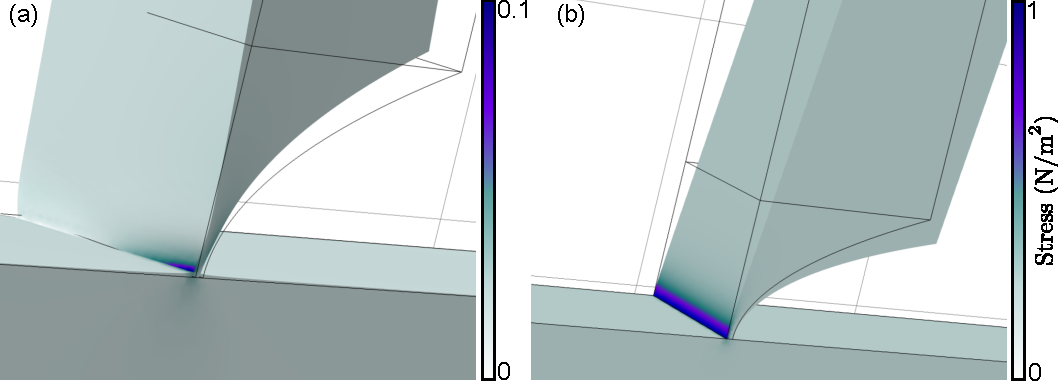
\includegraphics[width=0.95\textwidth]{../figures/bridge_stress.pdf}
    \caption[Stress simulation of a cantilever bridge]{COMSOL simulation of a diamond cantilever with bridge structure attaching to a larger support structure. The bridge is designed such that a sharp angle is present only at the junction, creating a likely fracture point. The width of the bridge at the junction is \qty{500}{\nano\meter}. (a) The stress response of the bridge for a force perpendicular to the cantilever plane, (b) and for a force along the cantilever plane. The stress is significantly higher for the in plane axis breaking force.}
    \label{fig:bridge_snap}
\end{figure}

\begin{figure}[h]
    \centering 
    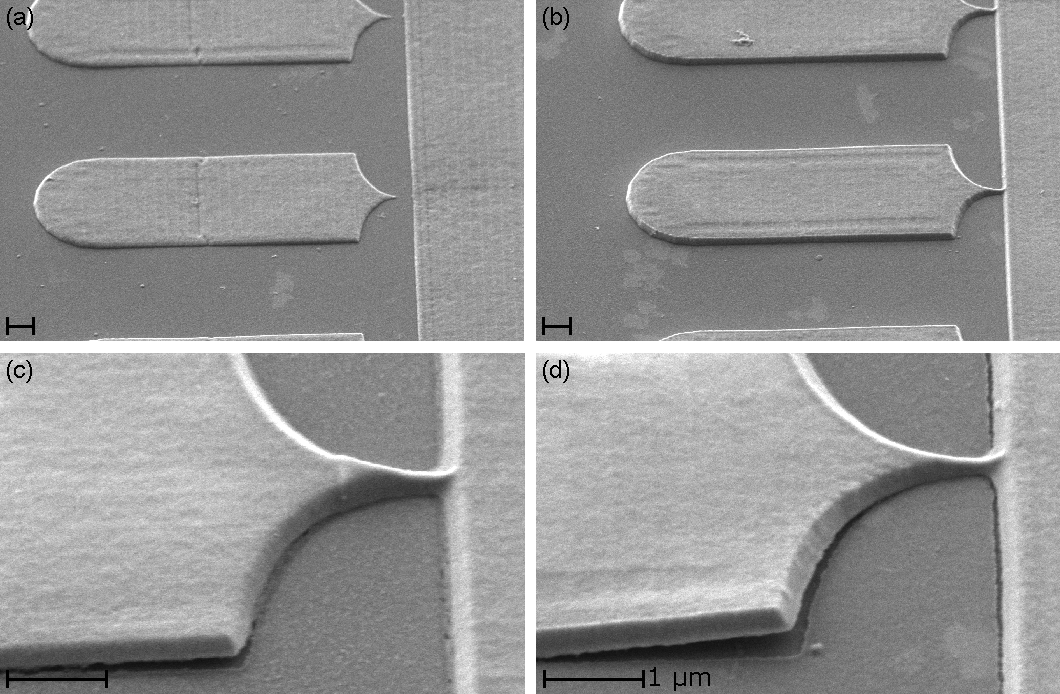
\includegraphics[width=0.95\textwidth]{../figures/medusa_cantiA.pdf}
    \caption[Proximity exposure effects on Medusa]{Exposures of Medusa for various designs. (a) Design with uniform dose for the entire cantilever. The loss of the bridge is seen due to underexposure. (b) Design with proximity effect correction (PECS). The bridge is exposed with smaller cells of higher dose factors. (c) PECS is done by a simple copy of the isolated bridge structure over the cantilever design, effectively a double exposure. Note the difference in thickness present, which can be transferred to the diamond. (d) PECS is done using nano-PECS (Raith Systems) software that calculates the dose factor for the design. There is also visible scumming\cite{rooksHSQStorage} and poor adhesion of the Medusa to diamond, although an adhesion promoter is used (SurPass 3000, DisChem).}
    \label{fig:medusa_cantiA}
\end{figure}

\subsection{Back side metallization}\label{app:metallization}


\subsection{Metal deposition - selectivity and effective deposition rate}\label{app:metal_deposition}